\section{增长动力:顺应时代趋势,做精团队合作}
Atlassian成长至今,增长的来源既有敏捷开发普及、全面上云的时代红利,也有公司内部持续迭代、打磨团队合作的内驱动力。
\begin{figure}[H]
    \caption{Atlassian与美股SaaS指数复盘}
    \begin{center}
        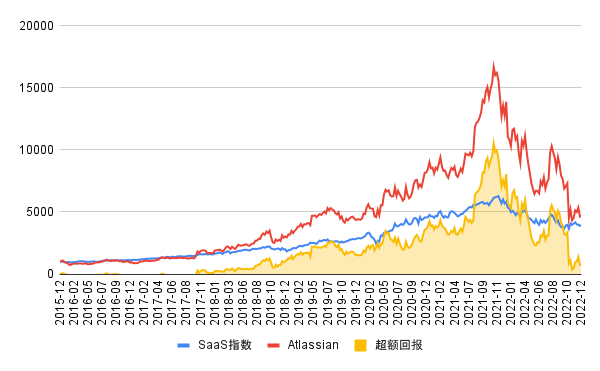
\includegraphics[width=0.9\linewidth]{img/excessreturn.png}
    \end{center}
    \footnotesize{资料来源:Wind。注:指数与股价初值归一为1000。}
\end{figure}

\subsection{时代的\texorpdfstring{$\beta$}——敏捷开发与DevOps、全面上云、疫情催化}
\textbf{软件工程经历了瀑布式开发、敏捷开发与DevOps三个阶段,Atlassian抓住了后两个阶段的时代机遇}。具体而言:
\begin{enumerate}
    \item 及时响应敏捷开发。1980年代的传统瀑布模型流程有严格的先后之分,自上而下的流程像极了瀑布的下落,但是新需求的增加会打乱整个发布节奏。2001年敏捷开发被提出,将软件项目需求分成多个迭代,且每个迭代成果在完成开发、测试、反馈等环节后都可以进行交付。Atlassian抓住了时代的历史机遇,于2002年便推出了Jira。高效的敏捷开发迅速在各大公司被采用,而随着敏捷开发进一步地普及,Atlassian打造出了Jira的口碑。
    \item 修正敏捷开发的缺陷。敏捷开发认为工作的软件高于详尽的文档,忽视了文档的重要性。Atlassian的解决方案是2003年推出的Confluence,与Jira高度的集成。此外由于敏捷开发是迭代式开发,在每个迭代中都有一个小型的、完整的开发流程,因此开发成本高。Atlassian的解决方案是2008年收购Bitbucket,覆盖开发全流程提升生产力。
    \item 云化提升DevOps水平。2009年针对敏捷开发的痛点,DevOps概念被提出。DevOps统一软件开发和运维,实现高度的自动化,监控软件制造过程中的各个阶段的数据,包括集成,测试,发布,部署基础设施管理。Atlassian在此时通过上云实现了持续集成/持续交付(CI/CD),并通过不断扩展产品外延,如Jira Service Management等协助企业内部的沟通管理。
\end{enumerate}
\begin{figure}[H]
    \begin{center}
        \begin{minipage}{0.3\linewidth}
            \caption{1980s瀑布开发}
            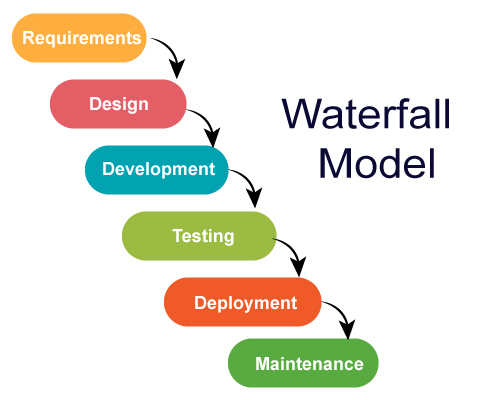
\includegraphics[width=\linewidth]{img/waterfall.png}
        \end{minipage}
        \begin{minipage}{0.3\linewidth}
            \caption{2000s敏捷开发}
            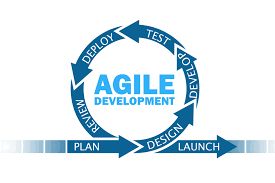
\includegraphics[width=\linewidth]{img/agile.png}
        \end{minipage}
        \begin{minipage}{0.3\linewidth}
            \caption{2010s DevOps}
            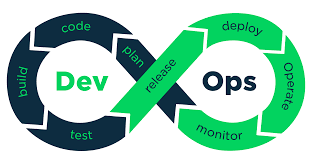
\includegraphics[width=\linewidth]{img/devops.png}
        \end{minipage}
    \end{center}
    \footnotesize{资料来源:51CTO}
\end{figure}

除此以外,企业上云也提升了Atlassian作为SaaS企业的价值,疫情带来的居家远程办公也进一步使Atlassian受益。大型企业上云重构了企业内部的沟通关系,以往利用邮件/人工/自建服务器追踪错误、维护文档移植到云上过于低效/复杂,云上的Jira、Confluence等在此时价值被企业所认知。远程办公对协作提出了更高的要求,Atlassian因此受益获得戴维斯双击。
% \begin{figure}[H]
%     \caption{软件开发越来越规范化,更倾向使用辅助工具}
%     \begin{center}
%         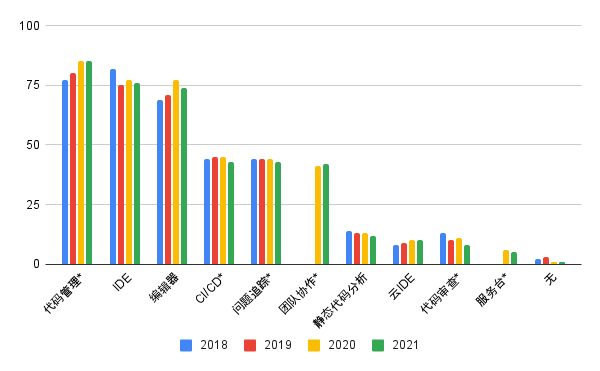
\includegraphics[width=0.9\linewidth]{img/tools.png}
%     \end{center}
%     \footnotesize{资料来源:Statista。注:标*为Atlassian覆盖的产品。}
% \end{figure}
\subsection{公司自身的\texorpdfstring{$\alpha$}——围绕团队合作打造Jira生态}
Atlassian CRO总结了其公司成长的飞轮模型\footnote{https://www.atlassian.com/blog/strategy/flywheel-effect-10-lessons},是三个组成部分构成的良性循环:吸引、参与、愉悦,即
\begin{enumerate}
    \item 通过优秀的产品吸引客户试用;
    \item 客户再试用的过程中感受到产品价值并付费;
    \item 付费的客户成为产品的推广者,将其在公司内容进行推广;客户在使用产品的过程中发现其他产品并试用;
\end{enumerate}
\begin{figure}[H]
    \caption{Atlassian总结的成长飞轮模型}
    \begin{center}
        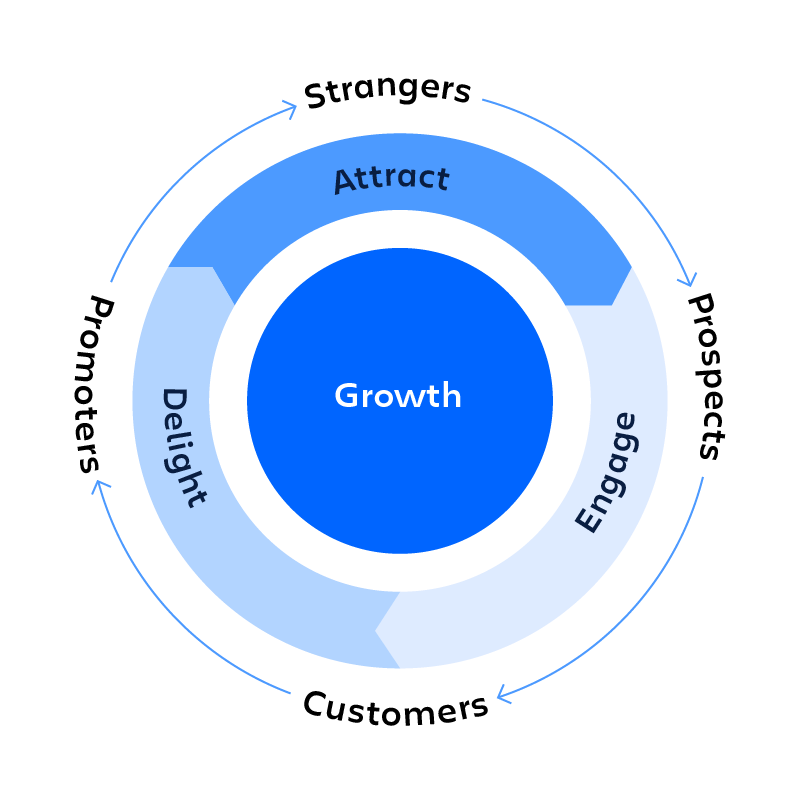
\includegraphics[width=0.8\linewidth]{img/flywheel.png}
    \end{center}
    \footnotesize{资料来源:Atlassian blog}
\end{figure}
\subsubsection{围绕核心产品Jira,专注于团队合作}
\textbf{飞轮的转动需要优秀产品的前提,Jira是一个复杂但优秀的软件}。Jira的复杂性来自于软件开发的复杂性,需要及时响应不同的需求、跟踪并分配质量参差不齐的issue、与复杂的代码有较高的集成度并能完成一定的自动化。这种复杂也给了技术人员自定义的权力,技术人员可以通过标准的或是自定义的工作流来处理软件开发中的实际问题,并获得效率上的提升。

\textbf{Atlassian专注于团队协作}。除收购的Trello外,Atlassian鲜有通用领域的产品,许多产品均是衍生自核心产品Jira的日常使用中,向外拓展进一步完善团队合作。典型例子如团队成立第二年便发布了Confluence,因为团队思考公司协作开发时需要做的所有事情,包括文档的集成。

\textbf{而对验证为无益于团队协作的产品,Atlassian会选择及时止损,并根据经验教训进行补充完善}。例如内部工作聊天软件Hipchat,Atlassian在Hipchat上复制了Jira复杂性,便于技术人员自定义但不利于一般地沟通,最终输给了Slack。Atlassian及时停止了该项目,并入股Slack在Slack中集成了Jira。

\textbf{高产品力也带动了Jira生态共荣}。Atlassian Marketplace年GMV约6亿美元\footnote{1月累计销售额达\href{https://www.atlassian.com/blog/announcements/shareholder-letter-q2fy22}{20亿},10月累计销售额达\href{https://www.linkedin.com/posts/amit-deshpande-785b3449_job-detail-atlassian-activity-6988005559119568896-mPG2?utm_source=share&utm_medium=member_desktop}{25亿}}。产品的高自定义能力吸引开发者自定义新的高效工作流并出售获利,实现生态内的共荣。
\subsubsection{免费与集成吸引潜在用户群}

\textbf{Atlassian的免费定价策略圈定了广泛的潜在客户群}。Atlassian成立之初软件公司大多依靠一次性付费许可,只有付费后才可以使用软件并且不可撤销。Atlassian则采用了免费试用的模式,这使得 Atlassian长期存续。如今Atlassian的许多产品如Jira都是对10人以下的小型团队、开源项目以及教育用途免费,吸引了广泛的用户。这些用户使用Jira等软件成为习惯时,成长后的公司或用户跳槽到的公司也会在这些用户的飞轮带动下使用 Atlassian的产品。

此外,Atlassian集成在各种编程所需的工具中,如聊天软件、IDE、代码托管网站等,进一步地扩大潜在用户群体。

\subsubsection{低成本营销带来成本优势}
\textbf{自助式销售降低了营销成本}。正如 Atlassian自己所说\footnote{\url{https://www.atlassian.com/blog/announcements/atlassian-founders-20-years-20-lessons}},软件应当被购买,而不是被出售。Atlassian 通过官网让用户自主选择产品套餐,在主页上有完全透明的价格体系,用户选择好产品类型、团队人数和部署方式后,就可以清楚地看到价格,并立即申请试用。这需要Atlassian持续降低销售中的摩擦,丰富自身文档的可用性和可达性,从而减少一对一地吸引潜在客户。

\textbf{依靠用户口碑宣传}。Atlassian 把 to B 的生意做成 to C,不仅产品是标准化 SaaS 软件,连销售方式也是如同电商一般,在用户之中的口碑是 Atlassian 最有力的武器,许多使用过Atlassian 产品的个人用户都愿意为其站台,达成飞轮效应。

\textbf{低成本的营销带来了成本优势}。在1Q23电话会上被问及产品的竞争优势时,管理层指出相较于其他产品, Atlassian的价格低于绝大多数替代品,较低的营销成本为有吸引力的价格打下了基础。

\subsubsection{研发驱动,鼓励创新的文化}

\textbf{Atlassian是一家研发型公司}。Atlassian研发费用率维持在45\%以上,横向对比其他SaaS公司也位于前列。高研发支出使得出品的软件大多为精品,增强用户口碑。

\textbf{Atlassian公司文化鼓励创新}。公司每年会举行hackathon ShipIt,鼓励员工和生态内的合作伙伴抽出一天时间尝试新想法并付诸实践。JSM的前身Jira 服务台便是ShipIt的产品。
\begin{figure}[H]
    \caption{Atlassian横向比较研发费用率也很高}
    \begin{center}
        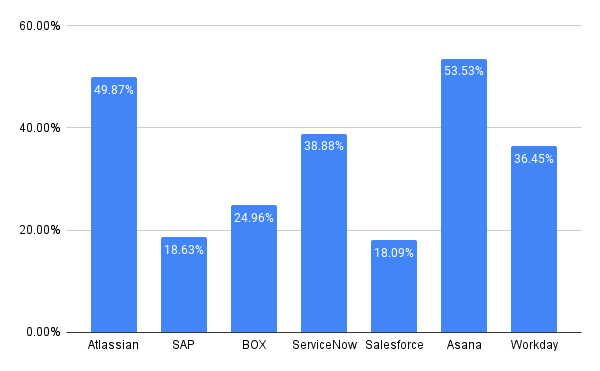
\includegraphics[width=0.9\linewidth]{img/RD.png}
    \end{center}
    \footnotesize{资料来源:Wind}
\end{figure}
